\section{Introduction}

Critical honeycomb walks and polygons have positive geometric weights,
while exact transfer representations of their partitions can involve
signed auxiliary weights. We study how cancellations in such a
representation can be controlled well enough to prove power laws. Our
principal cylinder estimate yields a planar nesting exponent. An
independent boundary calculation supplies the normalization and visit
identity needed for conclusions about lengths of finite chords. A separate
two-bond calculation controls the length-square mass of planar polygons.

\subsection{The physical observables}

Let $\mathbb H$ be the honeycomb graph formed by the centers of the
triangles of a regular triangular tessellation of side length one.
Planar distances and diameters refer to this Euclidean embedding.
A port is the midpoint of a tessellation side on the boundary of a region.
A port-to-port walk traverses distinct triangle centers and stops at its
first boundary exit. If it visits $N$ centers, its critical weight is
$x^N$, where
\[
 x=(2+\sqrt2)^{-1/2}.
\]
For a closed polygon, $|\lambda|$ denotes its number of bonds, which is
also its number of vertices. All polygon sums below count unoriented,
unrooted cycles. A sum modulo translations counts each lattice
translation class once.
Two cycles are incompatible if they share a vertex; a cycle is
incompatible with itself. Their basic pair weight is
$x^{|\lambda|+|\lambda'|}$.

Identify horizontal tessellation coordinates modulo $M=2m$, with $m$
even. Mark the face centers $O=(0,0)$ and $O'=(m,0)$ on a horizontal cut.
Call the $2m$ tessellation sides along this cut its sites. Write $A$ for
the $m$ sites from $O$ to $O'$ in eastward order and $B$ for the remaining
$m$ sites.
Let $G_m(g)$ be the sum over collections of disjoint simple cylinder
cycles, each separating $O$ from $O'$, with weight
\[
 \prod_{\lambda}g x^{|\lambda|}.
\]
The empty collection contributes one; Figure~\ref{j:fig-cylinder} shows
the two site intervals. The cylinder is infinite in the
vertical direction; equivalently take increasing finite cylinders with
closed rims, meaning that every port on either rim is unused. The proof
below establishes finiteness and identifies this limit. Because each
cycle crosses the cut between the marks, $G_m$ is a polynomial in $g$
of degree at most $2m$.

\begin{figure}[ht]
\centering
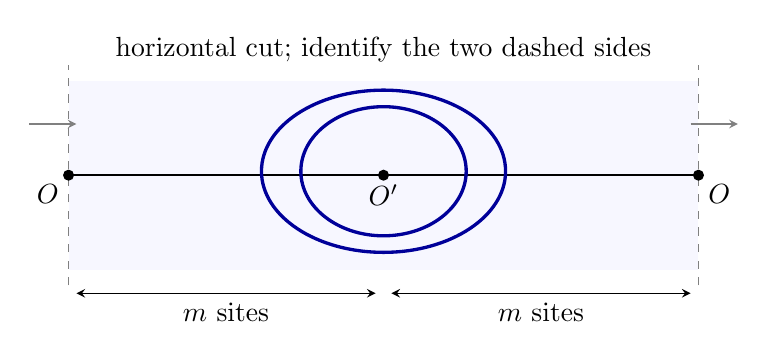
\begin{tikzpicture}[x=1cm,y=1cm,>=stealth]
 \fill[blue!3] (0,-1.2) rectangle (8,1.2);
 \draw[dashed,gray] (0,-1.4)--(0,1.4);
 \draw[dashed,gray] (8,-1.4)--(8,1.4);
 \draw[thick] (0,0)--(8,0);
 \fill (0,0) circle(2pt) node[below left] {$O$};
 \fill (4,0) circle(2pt) node[below] {$O'$};
 \fill (8,0) circle(2pt) node[below right] {$O$};
 \draw[<->] (.1,-1.5)--(3.9,-1.5) node[midway,below] {$m$ sites};
 \draw[<->] (4.1,-1.5)--(7.9,-1.5) node[midway,below] {$m$ sites};
 \draw[very thick,blue!60!black] (4,.05) ellipse (1.05 and .82);
 \draw[very thick,blue!60!black] (4,.05) ellipse (1.55 and 1.03);
 \draw[->,gray] (-.5,.65)--(.1,.65);
 \draw[->,gray] (7.9,.65)--(8.5,.65);
 \node at (4,1.6) {horizontal cut; identify the two dashed sides};
\end{tikzpicture}

\caption{The balanced cylinder, shown cut open along its seam. The two
marks split a period into equal site lists. The drawn nested cycles
separate the marks; the definition also permits noncontractible
separating cycles. The drawing is schematic rather than a lattice
embedding.}\label{j:fig-cylinder}
\end{figure}

For a regular tessellation hexagon $D_R$ of integer side length $R$, let
$\mathcal Z(R)$ be the partition of disjoint polygons contained in $D_R$
and surrounding its central face, each weighted by $2x^{|\lambda|}$;
the empty collection contributes one. Let $\mathcal C_R$ consist of
the ordered first-exit chords of $D_R$ whose diameter is at least $R/10$.
Both boundary ports are free: the sum includes every starting port and
every possible first-exit port, retaining the direction from start to
exit. Define the finite partition and probability law by
\[
 Z_R^{\rm chord}=\sum_{\gamma\in\mathcal C_R}x^{N(\gamma)},\qquad
 \mathbb P_R^{\rm chord}(\gamma)
   =\frac{x^{N(\gamma)}}{Z_R^{\rm chord}}\quad(\gamma\in\mathcal C_R).
\]

For a positive quantity $F(R)$, the notation $F(R)=R^{a+o(1)}$ means
$\log F(R)/\log R\to a$. An upper bound $F(R)\le R^{a+o(1)}$ means
that for every $\epsilon>0$ it is at most $C_\epsilon R^{a+\epsilon}$.
Uniform occurrences of this notation have constants and thresholds
independent of the indicated geometric data.

\begin{theorem}[Cylinder pressure and planar nesting]\label{j:cylinder}
As $m\to\infty$ through even integers,
\[
 G_m(2)=m^{1/6+o(1)},\qquad
 -\left.\frac{d^2}{dg^2}\log G_m(g)\right|_{g=0}=O(\log m).
\]
The derivative is the total basic weight of ordered incompatible pairs
of separating cycles, including a cycle paired with itself. Locally
uniformly for complex $\Theta$ with $|\Re\Theta|<\pi$,
\[
 |G_m(2\cos\Theta)|
 \le m^{\Re(1/6-2\Theta^2/(3\pi^2))+o(1)}.
\]
The planar partition satisfies $\mathcal Z(R)=R^{1/12+o(1)}$ as $R$ tends
to infinity through integers.
\end{theorem}

\begin{theorem}[Finite chords and marked polygons]\label{j:hexagon}
For the chord law just defined,
\[
 Z_R^{\rm chord}=R^{3/4+o(1)},\qquad
 \mathbb E_R^{\rm chord}N=R^{4/3+o(1)}.
\]
Uniformly for honeycomb vertices $v$ at distance at most $R/10$ from the
hexagon center,
\[
 \mathbb P_R^{\rm chord}(v\in\gamma)=R^{-2/3+o(1)}.
\]
Furthermore, for planar polygons modulo lattice translations,
\begin{equation}\label{j:polygon-square}
 \sum_{\operatorname{diam}\lambda\le H}
      x^{|\lambda|}|\lambda|^2\le H^{2/3+o(1)}.
\end{equation}
\end{theorem}

The chord conclusions describe this finite law, which is normalized
over all lengths allowed by the domain and the diameter cutoff. The
visit estimate concerns the stated bulk vertices. The final inequality
sums closed polygons modulo translations. Its proof uses the
positive mass of single polygons passing through two specified bonds
on a tilted cylinder. Theorem~\ref{j:unequal}, stated at the start of
Section~\ref{c7:marked}, gives the precise restrictions on the two site
lists and the uniform estimate used for this purpose.

\subsection{Earlier work}

Nienhuis's analysis of the dilute $O(n)$ model predicted the
two-dimensional self-avoiding-walk exponents \cite{Nienhuis1982}.
The conventional spatial prediction is $\nu=3/4$: the mean-square
displacement of a uniform length-$n$ walk is expected to be
$n^{2\nu+o(1)}$ \cite[Equation~(8)]{DuminilCopinSmirnov2012}.
The reciprocal $1/\nu=4/3$ motivates the length exponent in our finite
chord law, whose normalization and boundary conditions are specified above.
Duminil-Copin and Smirnov proved the exact honeycomb connective constant
by a parafermionic local cancellation and a boundary-flux argument
\cite{DuminilCopinSmirnov2012}. Their theorem determines the critical
activity used here. The local cancellation also gives a positive bound
on a convex boundary partition; the chord law requires quantitative
control of the part carried by macroscopic exits.
The vanishing of critical bridge mass was proved by Beaton,
Bousquet-M\'elou, de Gier, Duminil-Copin and Guttmann
\cite{BeatonEtAl2014}. For honeycomb bridges, Glazman and Manolescu
subsequently obtained a logarithmic subsequence bound. For their specified
columnwise rhombic half-plane tilings they also proved invariance of boundary
two-point functions \cite[Theorem~1 and Proposition~1.1]{GlazmanManolescu2017}.
Krachun and Panagiotis obtained a polynomial upper bound on the critical
bridge partition and used it to prove quantitative sub-ballisticity for
uniform length-$n$ honeycomb walks \cite{KrachunPanagiotis2026}.
These results concern distinct normalizations and precision levels;
our boundary proof establishes the radius-arch exponent with arbitrary
exponent slack.

The extension to rhombic weights connects this cancellation to
Yang--Baxter methods \cite{GlazmanManolescu2017}. Our local-weight and
fusion calculations keep the physical normalization explicit.

Grimm and Pearce developed a two-colour braid--monoid formulation of
dilute loop models and its Yang--Baxterization
\cite[Sections~4.2 and~4.6]{GrimmPearce1993}. The trigonometric weights
underlying the rhombic model trace back to Nienhuis
\cite{Nienhuis1990CriticalMulticritical,GlazmanManolescu2017}.
Finite-size corrections to periodic dilute-loop transfer-matrix spectra
have integrable-model predecessors \cite{ZhouBatchelor1997}.
For an open-strip dilute $O(1)$ model, Feh\'er and Nienhuis derive fusion
and current recursions \cite{FeherNienhuis2018}. Their current interpolation
in Section~6 uses rapidity-symmetry hypotheses stated in Section~5;
Appendix~E supplies a boundary fusion construction and explains why that
construction does not establish the current symmetries. The finite observable
here is different, and the symmetry within each of its two site groups is
proved directly. These earlier spectral and current formulas do not by
themselves identify its marked vacuum pairing or physical normalization.

The fermionic contractions and bosonic oscillator conversion belong to
the classical Wick and boson--fermion methods
\cite{Wick1950,Frenkel1981,FrenkelJingWang2000}; we compute their
twist, charge conventions and analytic limits in the normalization
needed here.

\subsection{Proof strategy}

The cylinder calculation begins by orienting occupied edges, with the
three states empty, forward and backward. Phases attached to turns,
seam crossings, and crossings of $A$ make the two orientations of a
loop cancel unless it separates the marks; a separating loop contributes
$g$. Long stacks with empty rims converge to vectors indexed by spin
configurations on the cut, whose pairing with the cut insertion gives
the partition. Finiteness of the total half-plane arch weight, proved in
Section~\ref{j:local}, justifies their limits. Section~\ref{c7:finite}
then uses local exchange and fusion, a spectral projector, and
polynomial interpolation to obtain an exact finite sum over three-valued
site spins. It temporarily allows arbitrary consecutive lists $A,B$
and nonzero complex spectral variables at their sites. The balanced
honeycomb case is recovered by choosing equal list sizes and setting
all site spectral variables to $1$.

Individual terms in this spin sum have poles when these variables
coincide, although the combined expression is regular.
Sections~\ref{c7:contour} and \ref{c7:boson} replace the sum by contour
residues, separate the coincident sites, and express the contractions
as an angular fermion trace. Evaluating that trace in oscillator
coordinates gives a gas on a horizontal circle of auxiliary length
$T$. Its particles have two species, corresponding to $A$ and $B$,
and carry integer charges. The gas records a running total charge, an
integer that changes by minus each particle's total charge as particles are
crossed. The resulting weights are signed or complex.
For the balanced cylinder, the limit $T\to\infty$ is taken at each fixed
site count; the estimates in the site count come afterward.

Section~\ref{c7:stability} controls the absolute gas weights by a
quadratic cost in the number of particles in each box and in this
running total charge at box boundaries. Section~\ref{c7:compact} uses
this estimate to form a
compact block propagator, with a contracting auxiliary coordinate
carrying the interaction with earlier blocks exactly. The site factors
suppress certain particle types on a central interval of length
proportional to $\log m$. The limiting operator there omits those types;
the exterior operator allows all types. Their propagation rates therefore
produce a power of $m$.

The exterior operator still has signed weights, and its eigenvalues of
maximal modulus may have Jordan blocks. At fixed $m$, the finite identity
supplies a limit in which the perturbed trace minus the normalized
physical value times the unperturbed trace tends to zero.
After normalization by the spectral radius,
Lemma~\ref{j:trace-extraction} expands the $n$th power of the exterior operator into
factors $\zeta^n$ with $|\zeta|=1$, multiplied by polynomials in $n$,
and compares the polynomial coefficients in the trace identity. This
retains all Jordan terms and bounds the
physical value without dividing by a trace that may cancel.
The Pfaffian scalar computed in Section~\ref{c7:pfaffian}, the exact
normalization $G_m(0)=1$, and positivity of the coefficients of $G_m$
then give the cylinder exponent and the incompatible-pair bound.

The chord mean also requires the size of its own finite partition
$Z_R^{\rm chord}$. The local boundary balance controls the total exit
weight from a port; the chord partition requires the part carried by
macroscopic exits. Write $W_R$ for the total critical weight of
first-exit same-boundary arches in a half-plane bounded by a horizontal
tessellation line that start at a fixed port and reach distance at least
$R$. Section~\ref{c7:boundary}
determines $W_R$ by an argument depending on the local transfer
identities and independent of the compact propagator. The added-row
expansion identifies the derivative of a one-row auxiliary cylinder increment
with its circumference $M$ times the deficit left in the boundary
balance by half-plane arches that embed in that cylinder. Fusion gives
functional relations for the increment, which determine the derivative
through a positive density on ordered points $0<k_1<\cdots<k_M$ whose
additional factor is an average over unitary conjugates. Comparison
with ensembles whose orthogonal polynomials can be evaluated gives the
derivative exponent $3/4$. The resulting deficit recovers the full
mass in the boundary balance and gives an upper bound for the endpoint tail
and a lower bound for the radius tail. A wedge comparison supplies the
matching radius upper bound, hence $W_R=R^{-1/4+o(1)}$. A boundary
comparison transfers this estimate to macroscopic hexagon exits;
summing over the free starting ports gives
$Z_R^{\rm chord}=R^{3/4+o(1)}$.

Proposition~\ref{j:visit} applies the boundary balance after removing
the triangle centered at a honeycomb vertex $v$ not adjacent to a
boundary port. It compares the raw weight of chords visiting $v$ with
the sum of the nesting partitions around its three incident
faces. For vertices within $R/10$ of the hexagon center, every such
chord meets the diameter cutoff when $R$ is sufficiently large.
Summing over vertices bounds the mean below by a constant times
$R^2\mathcal Z(\lfloor R/2\rfloor)/Z_R^{\rm chord}$ and above by a
constant times $R^2\mathcal Z(3R)/Z_R^{\rm chord}+R$; the additive term
accounts for vertices adjacent to boundary ports.
Section~\ref{c7:localization} uses the $O(\log m)$ incompatible-pair
bound to show that the sum of $x^{|\lambda|}$ over all noncontractible
separating cycles and all contractible cycles whose disk lifts are not
confined within a fixed multiple of $m$ around their enclosed mark is
$O(\sqrt{\log m})$. Their contribution costs a subpower factor.
The remaining cycles lift near one of the marks, giving upper and
lower comparisons of $G_m(2)$ with products of planar nesting
partitions at comparable radii. This gives
the exponent $1/12$; the visit comparison and chord normalization then
give the mean and bulk-visit exponents.

The length-square mass is handled through the positive sum of
$x^{|\lambda|}$ over single polygons using two specified bonds. After
a lattice rotation or reflection, the marked estimate in
Theorem~\ref{j:unequal} applies to cylinders whose cuts use horizontal
tessellation steps and steps tilted by $\pi/3$. Both marked bonds cross
horizontal steps, and the proportions of the two directions in each
unmarked list satisfy the restrictions in that theorem.
Sections~\ref{c7:marked}--\ref{c7:shifted} derive the matrix and
horizontal representations of this two-bond sum, including their
scalar normalization and uniform suppression for those lists. If
their sizes are $m$ and $n$, the two suppression
intervals have lengths proportional to $\log m$ and $\log n$. On the
parts covered by only the longer interval, the mixed propagator allows
all types in one species and only the unsuppressed types in the other.
Section~\ref{c7:mixed} bounds this propagator by a separate calculation
with one species. Monotonicity of the running total charge
controls the central region where both suppressions act. The final
counting argument sums the marked estimate over selected bond pairs whose
displacements fit these cuts and
separately bounds polygons for which too few such pairs are available.
This proves
\eqref{j:polygon-square}.
